\section{Sample of Black Holes}

\label{sec:sample}The BH population in Illustris was analysed using 
the low resolution simulation at a redshift of $z=0$. The Illustris 
simulation gives the mass ($M$) and accretion rate ($\dot{M}$) for each BH. We first 
eliminate all BH particles with $M=0$ or $\dot{{\rm M}}=0$, which 
we assume to be unphysical. We will hereafter refer to the remaining 
population (admittedly somewhat anomalously) as the Full Illustris-2 
Black Hole Sample. We argue that if accretion rate and X-ray luminosity 
are indeed linearly related, accretion rates on the order of 
$\sim10^{-15.7}M_{\odot}s^{-1}$ and lower should not be detectable in 
the X-ray bands at cosmological distances. To justify this, we examine 
the typical energy output of an SMBH (as stated above, 
$\sim10^{42}\,{\rm ergs}\,{\rm s^{-1}}$). Assuming that the thin-disk
approximation with 10\% efficiency is correct (see \ref{sec:analysis}
for a full discussion), one can show that a black hole accreting at 
such a low rate would have an energy output of on the order 
$\sim10^{37}\,{\rm ergs}\,{\rm s^{-1}}$. This fact, with the 
additional note that the presence of the low-accreting population 
skews the $M-\dot{M}$ fit severely, makes a compelling case for
eliminating that population.

We accomplished this by first noting that the main sequence of black
holes follows roughly a log-normal distribution in accretion rate
space, centered around approximately $\dot{M}_{BH}=10^{-12.5}M_{\odot}/s$.
However, there also exists a small, secondary population centered
around approximately $\dot{M}_{BH}=10^{-15.7}M\odot/s$ (see Figure
\ref{fig:bhpop_mdot}). To produce a clean sample of accreting black
holes, we fit the Full Sample with two Gaussian profiles (in $\log\dot{M}$-space)
using astroML's one-dimensional Gaussian mixture \citep{vanderplas2012},
and require an accretion rate of $\ge10^{-15.7}\; M_{\odot}yr^{-1}$
(the arithmetic mean of the low-accreting sample). This yields a total
of $23,277$ for our final sample black holes with masses $5\times10^{4.3}M_{\odot}\le M_{BH}\le5.85\times10^{10}M_{\odot}$.
\begin{figure}
\centering{}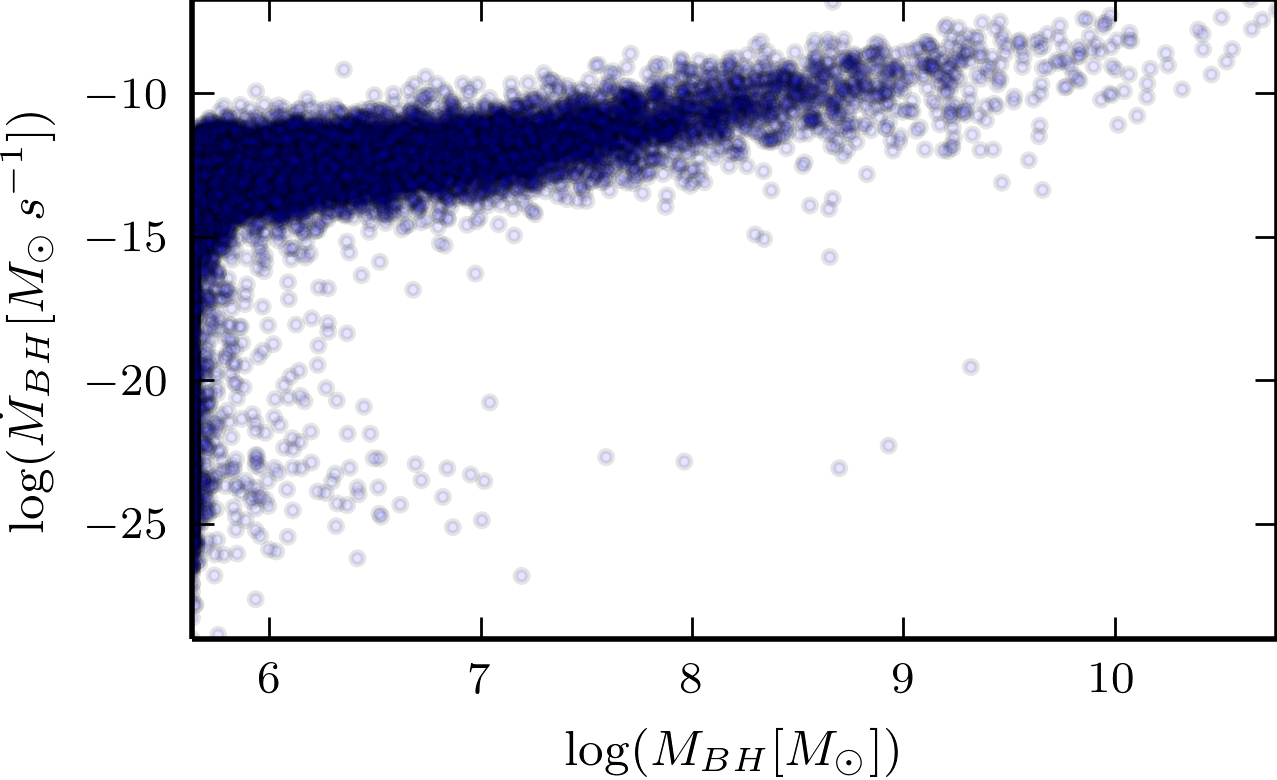
\includegraphics[clip]{Figures/Illustris2_bhpop_full}
\protect\caption{\label{fig:bhpop_full}The full Illustris-2 black hole sample in mass-accretion
rate space. Each light blue dot represents a single black hole with
mass in units of $M_{\odot}$ and accretion rate in units of $M_{\odot}s^{-1}$.}
\end{figure}
\begin{figure}
\centering{}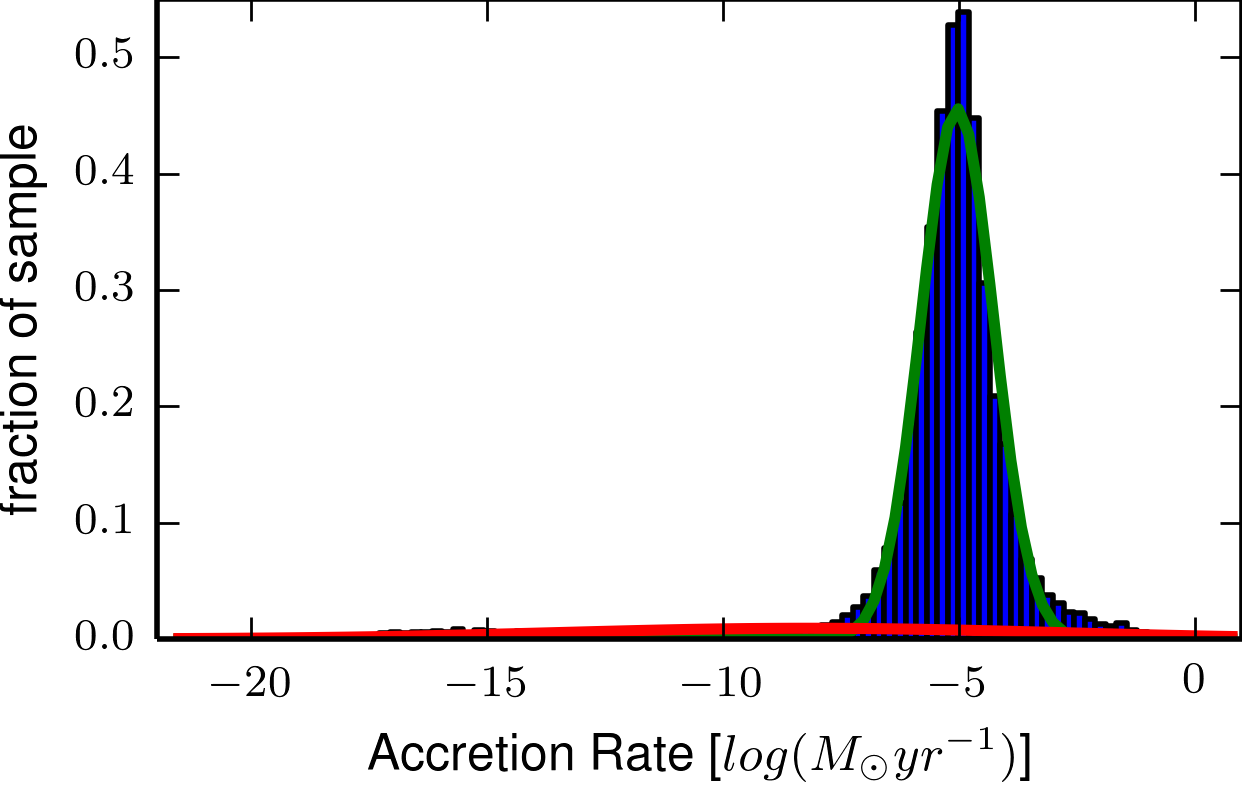
\includegraphics[clip]{Figures/Illustris2_bhpop_mdot}
\protect\caption{\label{fig:bhpop_mdot}The Full Sample exhibits a weak, but noticeable
bimodality in accretion rate space. We fit two log-normal distributions
to the raw distribution. The green Gaussian profile denotes the high-accreting
population, and the small, red Gaussian profile denotes the low-accreting
population. We impose a strict cutoff on the accretion rate at the
peak of the red profile, eliminating most of the anomalously low-accreting
population.}
\end{figure}
